\documentclass[12pt]{article}

\usepackage[utf8]{inputenc}
\usepackage{latexsym,amsfonts,amssymb,amsthm,amsmath}
\usepackage{float}

\setlength{\parindent}{0in}
\setlength{\oddsidemargin}{0in}
\setlength{\textwidth}{6.5in}
\setlength{\textheight}{8.8in}
\setlength{\topmargin}{0in}
\setlength{\headheight}{18pt}
\usepackage{graphicx}
\usepackage{tikz}

\usepackage{hyperref}
\hypersetup{
    colorlinks=true,
    linkcolor=blue,
    filecolor=magenta,      
    urlcolor=cyan,
    pdftitle={Overleaf Example},
    pdfpagemode=FullScreen,
}

\urlstyle{same}

\usepackage{caption}
\DeclareCaptionFormat{citation}{%
  \ifx\captioncitation\relax\relax\else
    \captioncitation\par
  \fi
  #1#2#3\par}
\newcommand*\setcaptioncitation[1]{\def\captioncitation{\textit{Source:}~#1}}
\let\captioncitation\relax
\captionsetup{format=citation,justification=centering}

\title{MATH1034OL1 Pre-Calculus Mathematics Notes from Sections 4.9, 3.6, 3.4 (Wednesday)}
\author{Elijah Renner}

\begin{document}

\maketitle

\vspace{0.5in}

\tableofcontents

\section{Factors of Polynomials}

If a polynomial has a zero of \(x=a\) whose multiplicity is \(b\), \((x-a)^b\) is a factor.

\section{Included Angles}

\begin{figure}[H]
	\centering
	\includegraphics[scale=1]{included.gif}
	\caption{Credit: \url{https://www.mathopenref.com/angleincluded.html}}
\end{figure}

\section{Law of Cosines}

We use the law of cosines to "solve" (find all angles and sides) of a triangle when we are given either a) three sides or b) two sides and the included angle.\\

Consider the triangle\\

\begin{figure}[H]
	\centering
	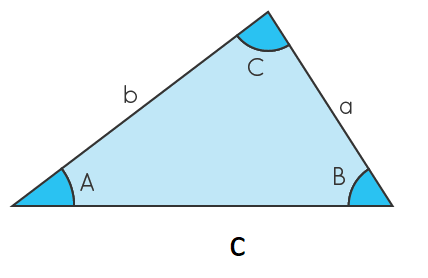
\includegraphics[scale=0.6]{abc.png}
	\caption{Credit: \url{https://www.cuemath.com/questions/for-triangle-abc-with-sides-a-b-and-c-the-law-of-cosines-states-the-following/}}
\end{figure}

with sides \(a\), \(b\), and \(c\) and angles \(A\), \(B\), and \(C\). We define the law\\

\[a^2=b^2+c^2-2bc\cos A\]

which can be rewritten by swapping any two of the variables:\\

\[b^2=a^2+c^2-2ac\cos B\]
\[c^2=a^2+b^2-2ab\cos C\]

These can also be rewritten algebraically to solve for angles \(A\), \(B\), or \(C\).

\section{Law of Sines}

The law of sines relates the proportions of sides to the sine values of the angles opposite the sides:\\

\[\frac{a}{\sin A}=\frac{b}{\sin B}=\frac{c}{\sin C}\]

The rule is useful when we are given either a) two angles and one side, or b) two sides and a non-included angle.\\

\section{Complex and Imaginary Numbers}

Let \(z\) be the complex number \(a+bi\). The conjugate of \(z\) is \(\bar{z}=a-bi\). One useful property to remember is that \(z\bar{z}\) is a real number.

\section{Asymptotes of Rational Functions}

\begin{figure}[H]
	\centering
	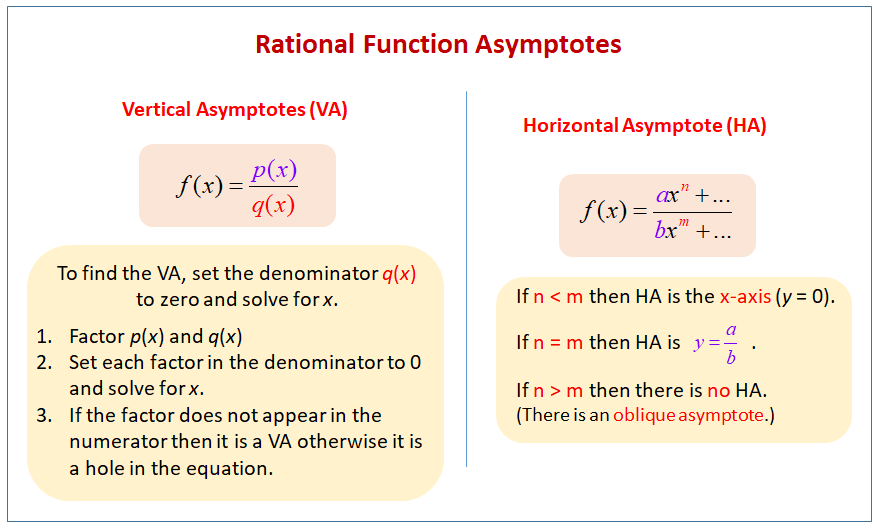
\includegraphics[scale=.75]{rational.png}
	\caption{Credit: \url{https://www.onlinemathlearning.com/rational-functions.html}}
\end{figure}

The x-intercepts of a rational function are the values that make the numerator equal to zero.\\

If the degree of the top polynomial is one greater than the bottom polynomial, there exists an oblique or slant asymptote:\\

\begin{figure}[H]
	\centering
	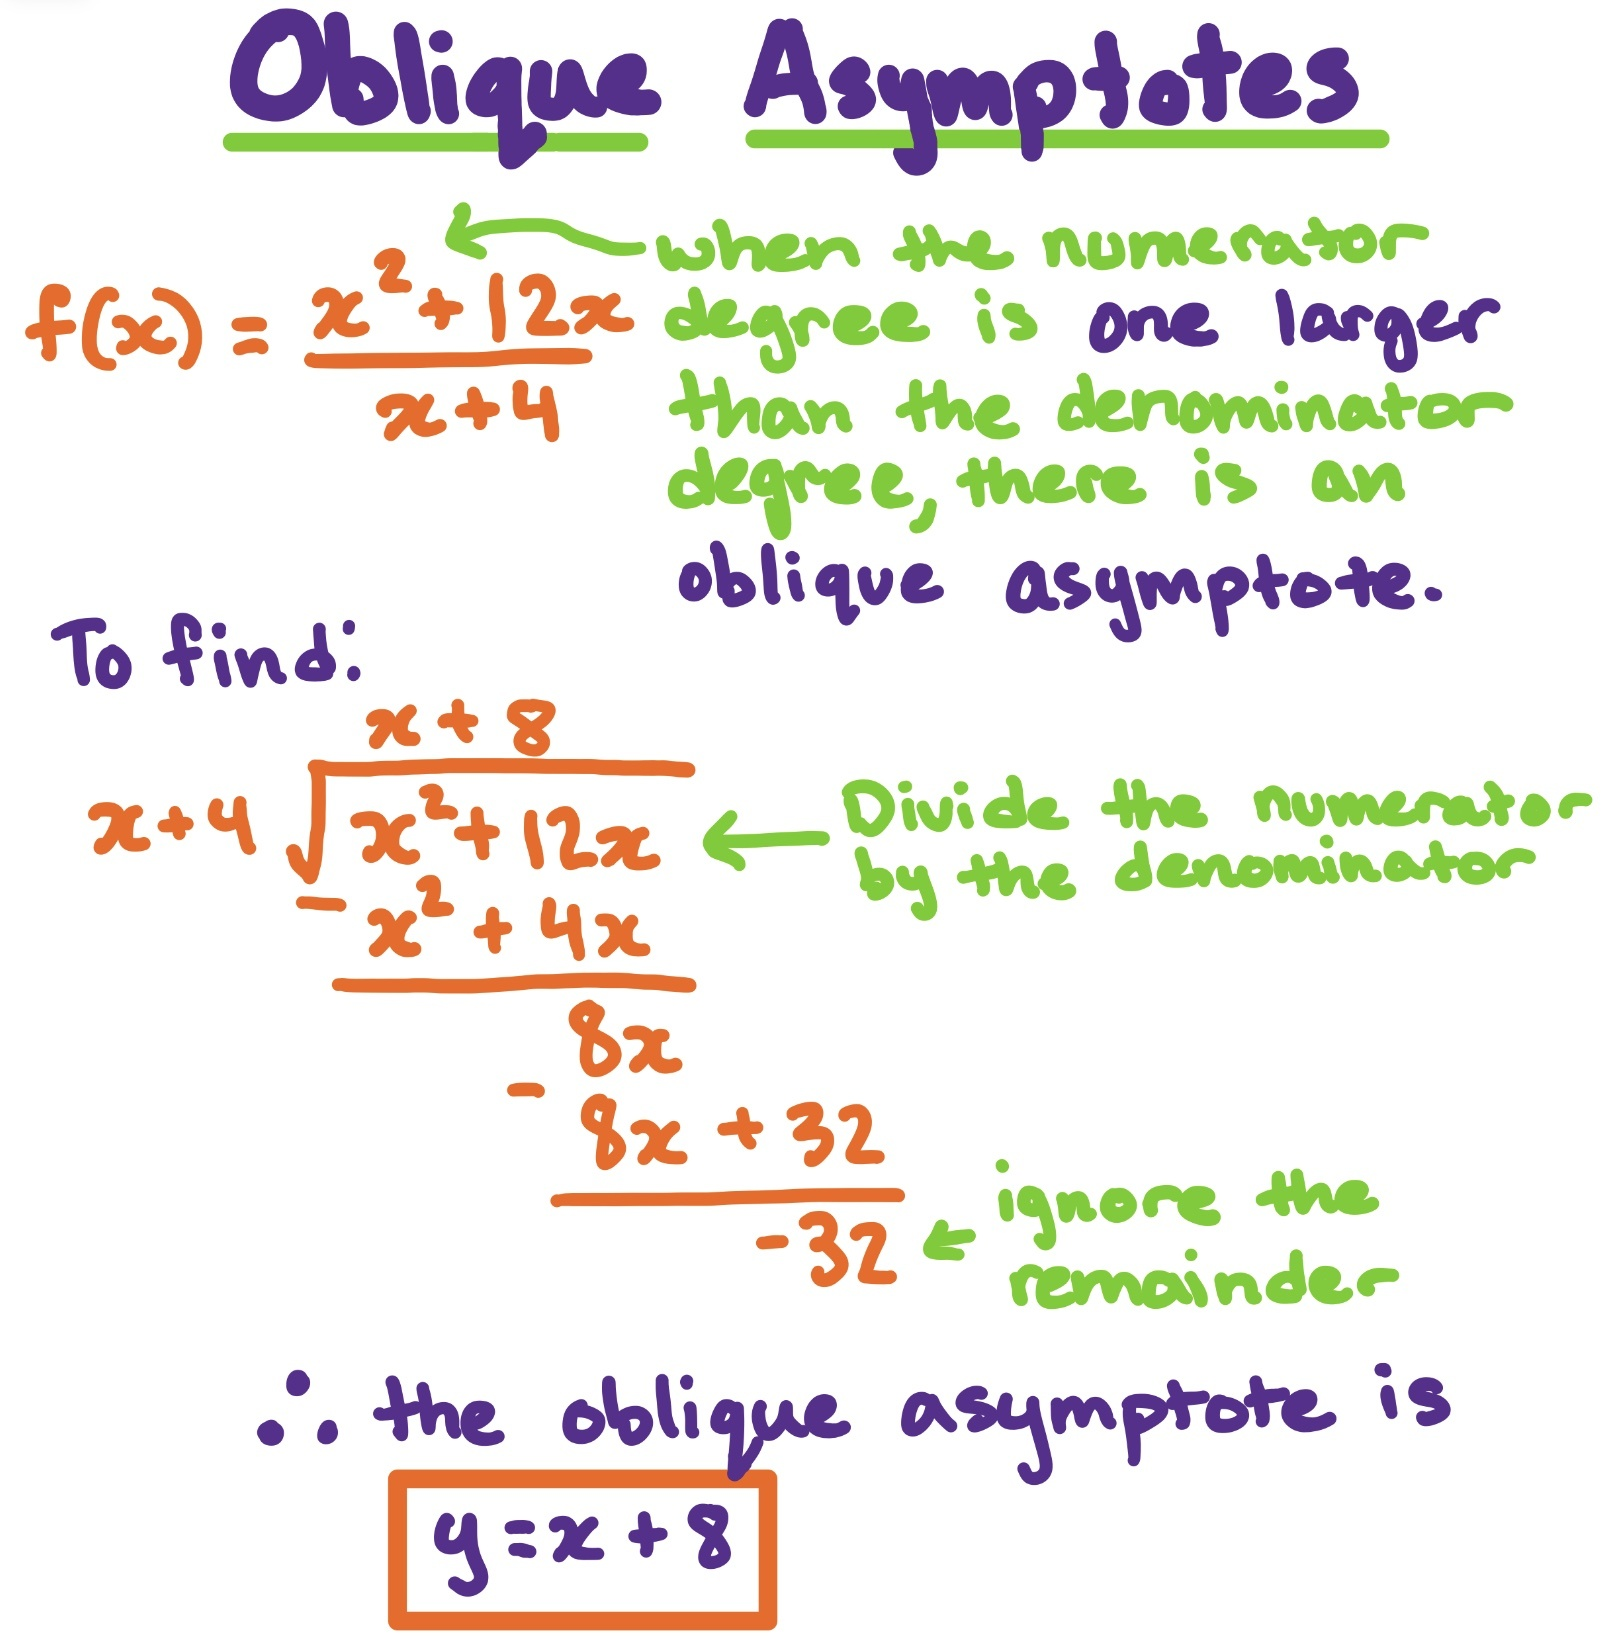
\includegraphics[scale=.2]{oblique.jpg}
	\caption{Credit: \url{https://www.expii.com/t/oblique-asymptotes-of-rational-functions-5138}}
\end{figure}

Some final notes about asymptotes:\\

Horizontal asymptotes and oblique asymptotes may be crossed by the rational function, but vertical asymptotes may not (because they're the values where the function is undefined).\\

To determine if some asymptote intersects a rational function, set them equal and look for a contradiction. If there isn't a contradiction, the rational function intercepts that asymptote at the value of x in that equality.\\

\end{document}